\chapter{Numerical results with \texorpdfstring{$\bigO(a)$}{O(a)}-improved Wilson fermions}
\label{ch:p2:numerics}

% \worktodo{
% * Numerical study
% 	* volume plots
% 	* Cost table
% 	* Additional plots
% 	* performance model
% 	* gauge variance
% * Sections
% 	* Ensembles and intro
% 	* Total variance
% 	* Gauge variance
% 	* Discuss relative variance plots
% 	* Discuss absolute variance plots
% 	* Discuss var-vs-srcs plots
% 	* Volume scaling
% 	* Cost
% }

\readit{1}

\worktodo{numerical study intro}

The numerical study was carried out using $\Nf=2$ flavours of non-perturbative $\bigO(a)$-improved Wilson-Clover fermions all with the same bare quark masses and lattice parameters.
They were generated starting from the CLS ensemble labelled F7~\cite{online:cls} in \cref{tab:mglma:ensembles}.
\begin{table}[t]
\centering
\begin{tabular}{ccccc}
\toprule
{ensemble}&
{$L_0 \times L^3$}&
{$L$ ($\mathrm{fm}$)}&
{$m_{\pi} L$}&
{\# configs} \\
\midrule
E7 & $64  \times 32^3$ & 2.1 & 2.9 & 100 \\
F7 & $96  \times 48^3$ & 3.2 & 4.3 & 100 \\
G7 & $128 \times 64^3$ & 4.2 & 5.8 & 100 \\
H7 & $192 \times 96^3$ & 6.3 & 8.6 & 5   \\
\bottomrule
\end{tabular}
\caption{\label{tab:mglma:ensembles}%
Ensembles used in the variance reduction study.
All lattices have a pion mass $m_{\pi} = $ \u{270}{\MeV} and a lattice spacing of $a = 0.0658(10)$ fm with $\Nf=2$ $\bigO(a)$-improved Wilson fermions with lattice coupling $\beta=5.3$, hopping parameter $\kappa=0.13638$ and $c_\mathrm{sw} = 1.90952$~\cite{online:cls,Jansen:1998mx}.
The largest ensemble H7 is only used to compute some variances which can be accurately determined from a few measurements.
F7 has been generated by the CLS initiative~\cite{online:cls}, while the others were generated by Tim Harris.
}
\end{table}
They all share the same pion mass of $m_{\pi} = $ \u{270}{\MeV} as well as the same lattice spacing $a = 0.0658$, but differ in volume.
The volumes span about two orders of magnitude from E7 to H7.
In this section, we demonstrate that the number of required low modes $\Nc$ for multigrid LMA is independent of the volume, where the gain in variance reduction remains constant.

For every ensemble in \cref{tab:mglma:ensembles} we investigated three estimators.
The first one is a plain stochastic estimator as described in \cref{sec:stochastic:prop} using spin-diagonal time-diluted random wall-sources with $\mathbb{Z}_2$ noise~\cite{ETM:2008zte} sampled randomly uniform over different time-slices.
This estimator is labelled ``stochastic'' in the plots.
Furthermore we ran a low-mode averaging estimator using a constant number of $\Nc=50$ low modes on all lattices labelled ``LMA''.
The eigen-eigen piece -- corresponding to the \Ln{1} term in multigrid parlance -- is evaluated exactly according to \cref{eq:Gconn:eigen-eigen}, whereas the remaining three terms are collected together, labelled \Ln{0} and evaluated stochastically~\cite{lynch2023} just as the plain stochastic estimator.
Finally we employ a multigrid LMA scheme with at least one non-trivial coarse lattice.
This class of estimators is labelled ``MG LMA''.
All the levels are usually evaluated stochastically just as the plain stochastic estimator, only exception is the coarsest level which is contracted exactly if its lattice was trivial~\cref{eq:mglma:coarsest:exact}.
Details about the LMA estimators can be found in \cref{tab:lma:estimators}.

For all ensembles and estimators that include low modes, we used a fixed number of $\Nc=50$ low modes of the Hermitian Dirac operator determined to a precision of $\norm{Q \evec - \lambda \evec} / \norm{\evec} \leq 10^{-12}$ using the library PRIMME~\cite{primme}.

\section{Methodology}
\label{sec:numerics:methodology}

% \worktodo{
% * How timers are taken. precision of timings
% * Energy measurements
% * averaged over 5 independent runs
% * what means "kernel"
% * NUMA placement, process pinning
% * CUDA-aware Cray MPICH 8.1.30 with GTL on top of Libfabric 1.15.2.0
% * CUDA 12.4 Driver version 550.54.15, GCC 13.2
% }

\tldr{how data was taken}
All time measurements were taken analogous to \cref{sec:perf:methodology}.
Estimators for the variances will be discussed in the main text as soon as they appear.
As estimator for the variance of the variance the method of jackknife resampling~\cite{efron1982jackknife,shao2012jackknife} was used throughout this document.

\tldr{machine we ran on}
Runs were performed on the machines
\begin{itemize}
    \item \emph{Piz Daint multicore} at CSCS, Switzerland, 2\x Intel\textsuperscript{\textregistered} Xeon\textsuperscript{\textregistered} E5-2695 v4 @ 2.10GHz (2$\times$ 18 cores, 64/128 GB memory)
    \item \emph{LUMI-C} at CSC, Finland, 2\x AMD EPYC\textsuperscript{\texttrademark} 7763 @ 2.45GHz (2\x 64 cores, 256-1024 GB memory)
    \item \emph{JUWELS} at Forschungszentrum Jülich, Germany, 2\x Intel\textsuperscript{\textregistered} Xeon\textsuperscript{\textregistered} Platinum 8168 @ 2.7 GHz (2\x 24 cores, 96-192 GB DDR4 memory @ 2666 MHz)
\end{itemize}


%\worktodo{
%   * methodology
%   * TTS meas. same as \cref{sec:perf:methodology}
%      * averaged over at least 5 independent runs
%   * estimators for variance follow
%      * variance of variance obtained with jackknife
%   * machines (old daint, juwels GPU, lumi-C) and MPI versions
%   * gcc version
%}

\begin{table}
\centering
\begin{tabular}{cccccc}
\toprule
         &  &       & \multicolumn{3}{c}{Block size $b_0/a\times(b_j/a)^3$} \\
\cmidrule(lr){4-6}
Ensemble &  Estimator & $\Nlvl$ & $\lvl=1$      & 2 & 3 \\
\midrule
E7 & LMA            & 2 & $64\times32^3$  & -              & -               \\
   & 2-level MG LMA & 2 & $8\times8^3$    & -              & -               \\
   & 3-level MG LMA & 3 & $8\times8^3$    & $64\times32^3$ & -               \\
\midrule
F7 & LMA            & 2 & $96\times48^3$  & -              & -               \\
   & 2-level MG LMA & 2 & $8\times8^3$    & -              & -               \\
   & 3-level MG LMA & 3 & $8\times8^3$    & $96\times48^3$ & -               \\
\midrule
G7 & LMA            & 2 & $128\times64^3$ & -              & -               \\
   & 2-level MG LMA & 2 & $8\times8^3$    & -              & -               \\
   & 4-level MG LMA & 4 & $4\times4^3$    & $8\times8^3$   & $128\times64^3$ \\
\midrule
H7 & LMA            & 2 & $192\times96^3$ & -              & -               \\
   & 2-level MG LMA & 2 & $8\times8^3$    & -              & -               \\
   & 4-level MG LMA & 4 & $4\times4^3$    & $8\times8^3$   & $192\times96^3$ \\
\bottomrule
\end{tabular}
\caption{
Details about all the estimators including low modes from \cref{fig:E7:var:vs:sources,fig:F7:var:vs:sources,fig:G7:var:vs:sources}.
For the different ensembles the table renders the number of multigrid levels, the block sizes used to generate the coarse lattices on each level.
% Block decompositions for the three estimators used in this work and the corresponding coarse-grid operators on levels $l$. 
When the block size matches the lattice volume, as is the case in the LMA schemes, no blocking is performed on that level.
%The coarsest level is not required to avoid blocking; for example the $\Nlvl=2$ MG LMA schemes terminate on a     block-projected level.
}
\label{tab:lma:estimators}
\end{table}

\section{Total variance}

The form of the total absolute variance depends on the number of stochastic sources $\Nst$ and includes a contribution from the stochastic noise.
It is defined as
\begin{equation} \label{eq:abs:variance}
\sigma_{G}^{2}(t) = \langle G(t)^{2} \rangle_{U} - \langle G(t) \rangle_{U}^{2} \;,
\end{equation}
where $G(t)$ is the stochastic estimator \cref{eq:stoch:Gij:final} with a single stochastic source $\Nst=1$ and $\langle \cdot \rangle_U$ is the average over gauge field configurations.

\section{Gauge variance}
\label{sec:numerics:gauge:variance}

Before we continue, we will discuss the gauge variance.
It is defined as the variance of the correlator $\mathcal{G}(t)$ averaged over the full spacetime lattice \cref{eq:G:corr:volume:averaged}.
It is the minimal variance given by
\begin{equation} \label{eq:var:gauge}
\sigma_{\mathcal{G}}(t) = \langle \mathcal{G}(t)^{2} \rangle_{U} - \langle \mathcal{G}(t) \rangle_{U}^{2} \;.
\end{equation}
The gauge variance is defined such that the variance of the sample mean over $\Nconf$ uncorrelated configurations would be $\sigma_{\mathcal{G}}/\sqrt{\Nconf}$.
We may use the samples from the pure stochastic estimator to estimate the variance
\begin{align}
\nonumber
&\sigma^{2}_{\mathcal{G}}(t) \approx
\frac{1}{\Nst(\Nst-1)} \sum_{m \neq n=0}^{\Nst-1}\\
\label{eq:appendix:gv:formula}
\qquad&\Big[ \langle C_m(t_m+t, t_m) C_n(t_n+t, t_n) \rangle_{U}
- \langle C_m(t_m+t,t_m) \rangle_{U} \langle C_n(t_n+t,t_n) \rangle_{U} \Big]
\end{align}
using \cref{eq:stoch:C:full:final}.
The total variance of the stochastic estimator was defined in \cref{eq:abs:variance} and in the limit of infinite stochastic samples it equals the gauge variance $\sigma_{\mathcal{G}}$,
\begin{equation} \label{eq:var:gauge:limit}
\lim_{\Nst \to \infty} \sigma_{G}(t) = \sigma_{\mathcal{G}}(t) \;.
\end{equation}
This limit is verified in \cref{fig:gauge:variance} for the E7 ensemble at time-slice $t \approx $ \u{1.3}{\femto \metre} for the isovector vector correlator up to \num{4096} stochastic sources.

\begin{figure}
\centering
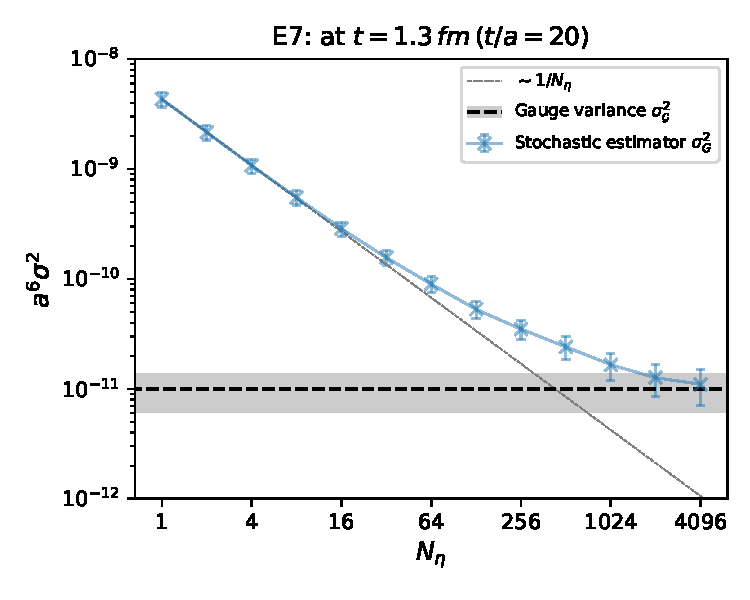
\includegraphics[width=0.5\linewidth]{\dir/img/gauge_variance}
\caption{
Verification of the limit \cref{eq:var:gauge:limit}.
The x-axis denotes the number of stochastic sources and the y-axis its corresponding variance.
The black dashed line with grey error bands represents $\sigma_{\mathcal{G}}(t)$ calculated using \cref{eq:appendix:gv:formula} and the blue solid line is the limit of $\sigma_{G}(t)$ as defined in \cref{eq:abs:variance}.
\takenfull
}
\label{fig:gauge:variance}
\end{figure}

\section{Relative variance}

We start with presenting relative variance plots for all ensembles in \cref{fig:rel:variance}.
The plots compare the LMA estimator with a 2-level MG LMA estimator~\cref{tab:lma:estimators}.
Shown on the y-axis is the relative variance of the corresponding level; the variance of one stochastic source normalized by the sum of variances of all levels, i.e.
\begin{equation} \label{eq:rel:variance}
\sigma_{rel}^{2} = \frac{\sigma^{2}}{ \sum_{\lvl} \sigma_{\Ln{\lvl}}^{2} } \in [0, 1] \;.
\end{equation}
This gives us an indication on how much variance contribution comes from which level, although without considering covariance among levels.
The variance of the sum of all levels -- the total variance, when summing -- is plotted as black solid line normalized by the sum of variances, highlighting that there is non-negligible covariance among the terms for the LMA data.
The only difference between the LMA and the MG LMA data in this plot is that for LMA the \Ln{1} coarse lattice is trivial, whereas for MG LMA it is not.
The effect of a non-trivial coarse grid -- as opposed to a trivial one -- reduces the variance contribution from the remaining piece on the fine grid by orders of magnitude on all four ensembles.

\Cref{fig:rel:variance} shows the $V^{2}$-problem of low-mode averaging, see \worktodo{V2-LMA-section}.
When looking at the LMA contributions from the smallest lattice E7 to the largest one H7, we observe a substantial increase in contribution from the remainder term (sum of rest-rest, rest-eigen and eigen-rest).
On the other hand in the MG LMA scenario, the variance contribution of the \Ln{0}-term stays negligible, even when holding the number of low modes constant.
This is thanks to keeping the block size fixed, resulting in a coarse lattice size that scales together with the volume.
This shows that the cost of sampling the data scales linear in the volume.

\begin{figure}
\centering

\subfloat[E7]{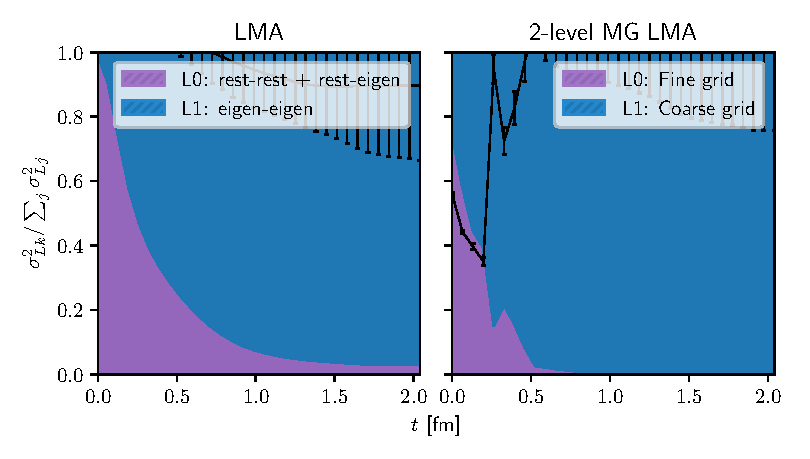
\includegraphics[width=0.49\textwidth]{\dir/img/E7/E7_rel_variance}\label{fig:E7:rel:variance}}
\hfill
\subfloat[F7]{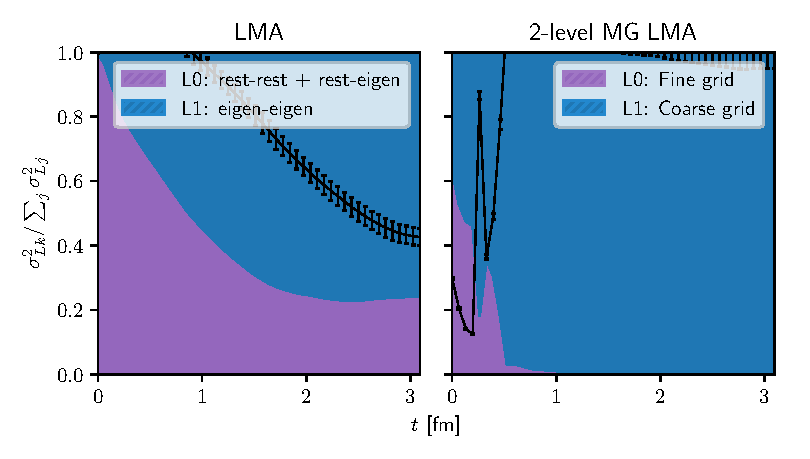
\includegraphics[width=0.49\textwidth]{\dir/img/F7/F7_rel_variance}\label{fig:F7:rel:variance}}

\subfloat[G7]{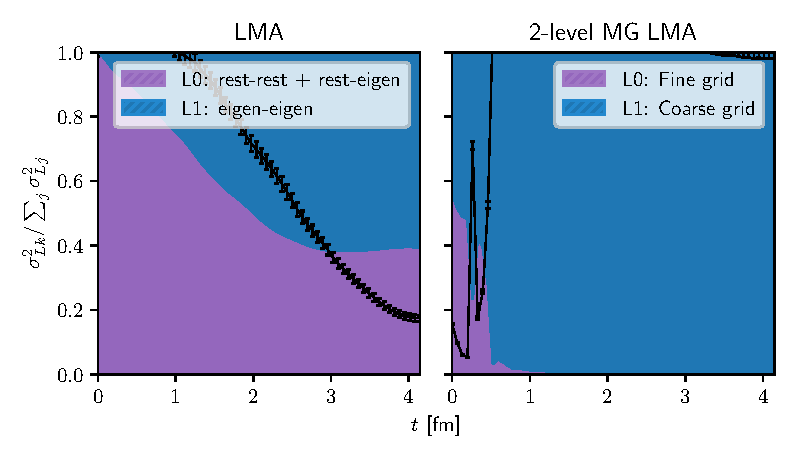
\includegraphics[width=0.49\textwidth]{\dir/img/G7/G7_rel_variance}\label{fig:G7:rel:variance}}
\hfill
\subfloat[H7]{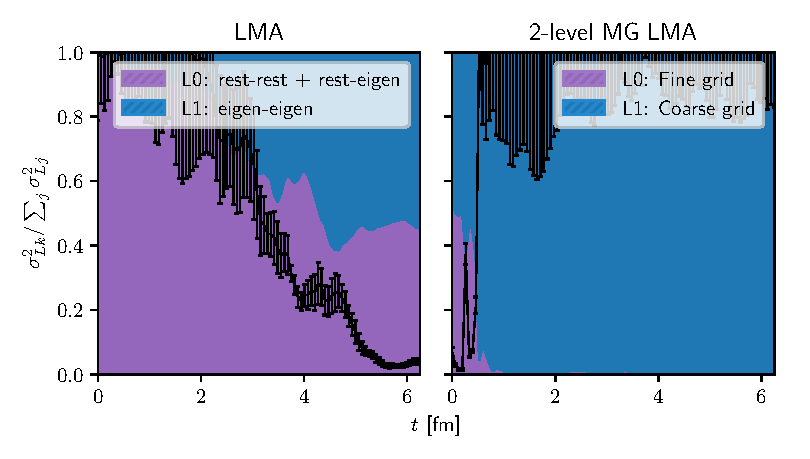
\includegraphics[width=0.49\textwidth]{\dir/img/H7/H7_rel_variance}\label{fig:H7:rel:variance}}

\caption{Relative variance \cref{eq:rel:variance} of one stochastic source of the two levels of LMA (left) and a corresponding 2-level MG LMA (right). The four groups of panels correspond to the four ensembles from \cref{tab:mglma:ensembles}. In all panels the purple and blue shaded regions denote fine-grid and coarse-grid contributions respectively. The solid black line shows the variance of the sum.}
\label{fig:rel:variance}
\end{figure}

\section{Absolute variance}

We now have a qualitative picture of the variance contributions.
Next, we will investigate the absolute variances of one single stochastic source in \cref{fig:E7:abs:variance,fig:F7:abs:variance,fig:G7:abs:variance,fig:H7:abs:variance}.
%The gauge variance of the full correlator is plotted on all panels as black dashed line with grey error band along with the plain stochastic estimator as blue solid line.
The plain stochastic estimator is plotted on all panels as blue solid line along with its gauge variance as black dashed line with grey error band.
Where the plain stochastic estimator gives us an upper bound for the variances, the gauge variance indicates the variance of the full volume averaged correlator, \cref{eq:G:corr:volume:averaged}.
Together they give us upper and lower bounds for the total variances.

Crucial for the analysis is the position of the \Ln{0}-variance, the yellow dashed line in all panels.
The closer it is to the gauge variance the better, since our ultimate goal is to push down all variances to the gauge variance.
When the gauge variance is reached, we have optimally used the available data.
In this endeavor clearly the fine-grid variance is the most expensive one to push down, as it involves expensive fine-grid inversions.

Pushing down the variance of the \Ln{0}-term can be achieved in multiple ways:
1) simply increasing the number of stochastic sources on the fine-grid, but that is associated with substantial cost,
2) increasing the number of low modes for the LMA estimator, but that increases the computational and memory cost even more,
or 3) employing a MG LMA scenario.

The plots show that we are able to push down the \Ln{0} variance to the gauge noise with only one single stochastic source on the fine-grid on all four ensembles irrespective or their volume.
Even though introducing stochastic noise, the \Ln{0} term is so subdominant in the relevant large time regime, that its total variance (stochastic and gauge) is below the gauge noise of the full correlator and therefore does only contribute negligibly when evaluated with a single stochastic source.
We note that for F7, \cref{fig:F7:abs:variance}, which seems to be a small exception, we did not use an ideal setup.
A block size of $8 \times 8^{3}$ for the first coarse level \Ln{1} is probably already too large, a better choice would be $6 \times 6^{3}$ on that lattice, whereas $4 \times 4^{3}$ is presumably too aggressive.

Of special interest is the smallest lattice E7 \cref{fig:E7:abs:variance}.
Low-mode averaging using \num{50} low modes is actually already beneficial on that lattice.
In a real world scenario one would probably increase the number a bit, but nevertheless the deflation is already working.
When comparing to MG LMA, clearly the non-trivial lattice still beats the trivial one.
We note that the subspace generated for the trivial lattice (LMA) is contained in the subspace of any non-trivial lattice (MG LMA).
This implies that a non-trivial coarse lattice will always have the better variance contribution than a trivial one assuming the same low modes were used in their construction.

On the larger lattices, G7 and H7 \cref{fig:G7:abs:variance,fig:H7:abs:variance}, we also show 4-level scenarios.
We found that on large lattices is it beneficial to dampen the cost of the possibly-very-large \Ln{1} term by deflating it again.
The coarsest level on these two lattices is trivial, i.e. corresponds to a layer of LMA.
Although this coarsest level does not contribute to the overall variance reduction, since a deflation of \num{50} low modes on these large lattices is simply not worth it.
This can be seen in the corresponding LMA plots (left panels), where the plain stochastic estimator basically coincides with \Ln{0}.
It clearly shows that the effect of the pure low mode deflation quickly becomes negligible as one increases the lattice volume keeping the number of low modes constant.

In order to enjoy the same variance contribution for LMA as on the smallest lattice E7, one has to increase the number of low modes proportional to the volume.
Such an increase would correspond to roughly $(\text{E7}, \text{F7}, \text{G7}, \text{H7}) \approx (50, 250, 800, 4000)$ low modes, only to obtain the variance contribution of \cref{fig:E7:abs:variance} right panel, which still does not push the \Ln{0} noise down to gauge noise.
The gauge noise level can be reached by either further increasing the number of low modes or by using a MG LMA scenario as in the right panels.

\begin{figure}
\centering
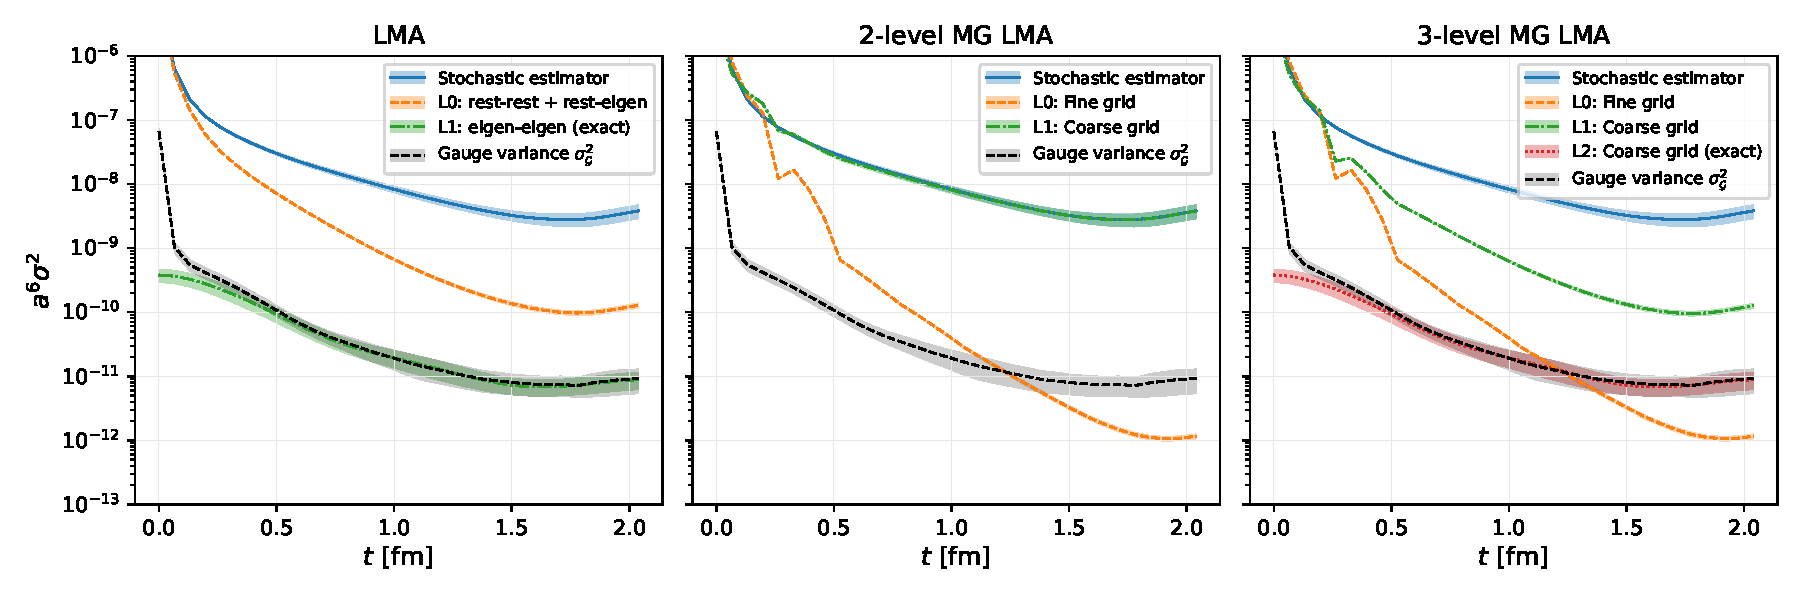
\includegraphics[width=1.0\linewidth]{\dir/img/E7/E7_abs_variance}
\caption{
E7: Absolute total variance \cref{eq:abs:variance} of a single stochastic source.
The left panel shows data for the LMA estimator, center and right show 2-level multigrid and a 3-level multigrid LMA estimator.
The blue solid line represents the pure stochastic estimator without any deflation and the black dashed line indicates the gauge variance of the full correlator. Both appear in all panels for comparison.
\takenpart
}
\label{fig:E7:abs:variance}
\end{figure}

\begin{figure}
\centering
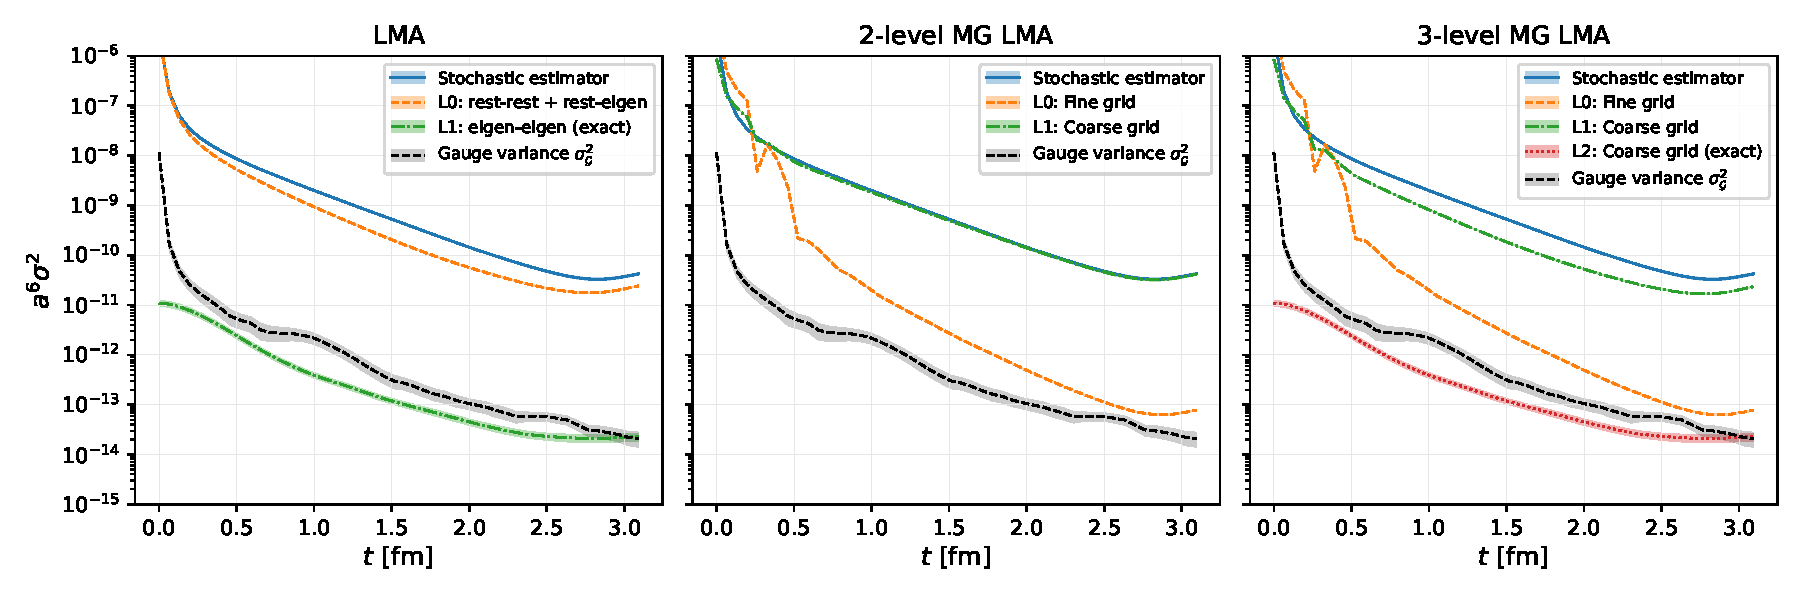
\includegraphics[width=1.0\linewidth]{\dir/img/F7/F7_abs_variance}
\caption{
F7: Absolute total variance \cref{eq:abs:variance} of a single stochastic source.
The left panel shows data for the LMA estimator, center and right show 2-level multigrid and a 3-level multigrid LMA estimator.
The blue solid line represents the pure stochastic estimator without any deflation and the black dashed line indicates the gauge variance of the full correlator. Both appear in all panels for comparison.
\takenpart
}
\label{fig:F7:abs:variance}
\end{figure}

\begin{figure}
\centering
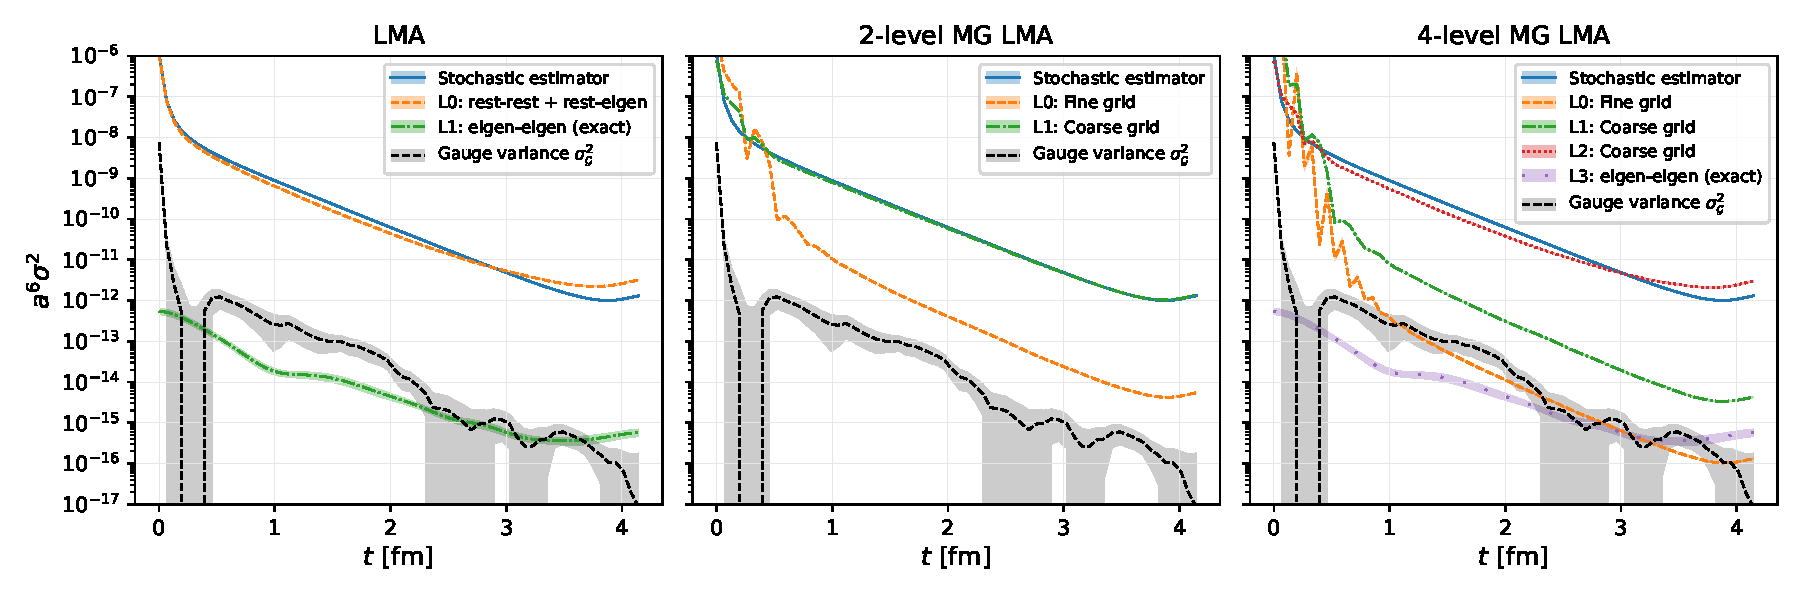
\includegraphics[width=1.0\linewidth]{\dir/img/G7/G7_abs_variance}
\caption{
G7: Absolute total variance \cref{eq:abs:variance} of a single stochastic source.
The left panel shows data for the LMA estimator, center and right show 2-level multigrid and a 4-level multigrid LMA estimator.
The blue solid line represents the pure stochastic estimator without any deflation and the black dashed line indicates the gauge variance of the full correlator. Both appear in all panels for comparison.
\takenpart
}
\label{fig:G7:abs:variance}
\end{figure}

\begin{figure}
\centering
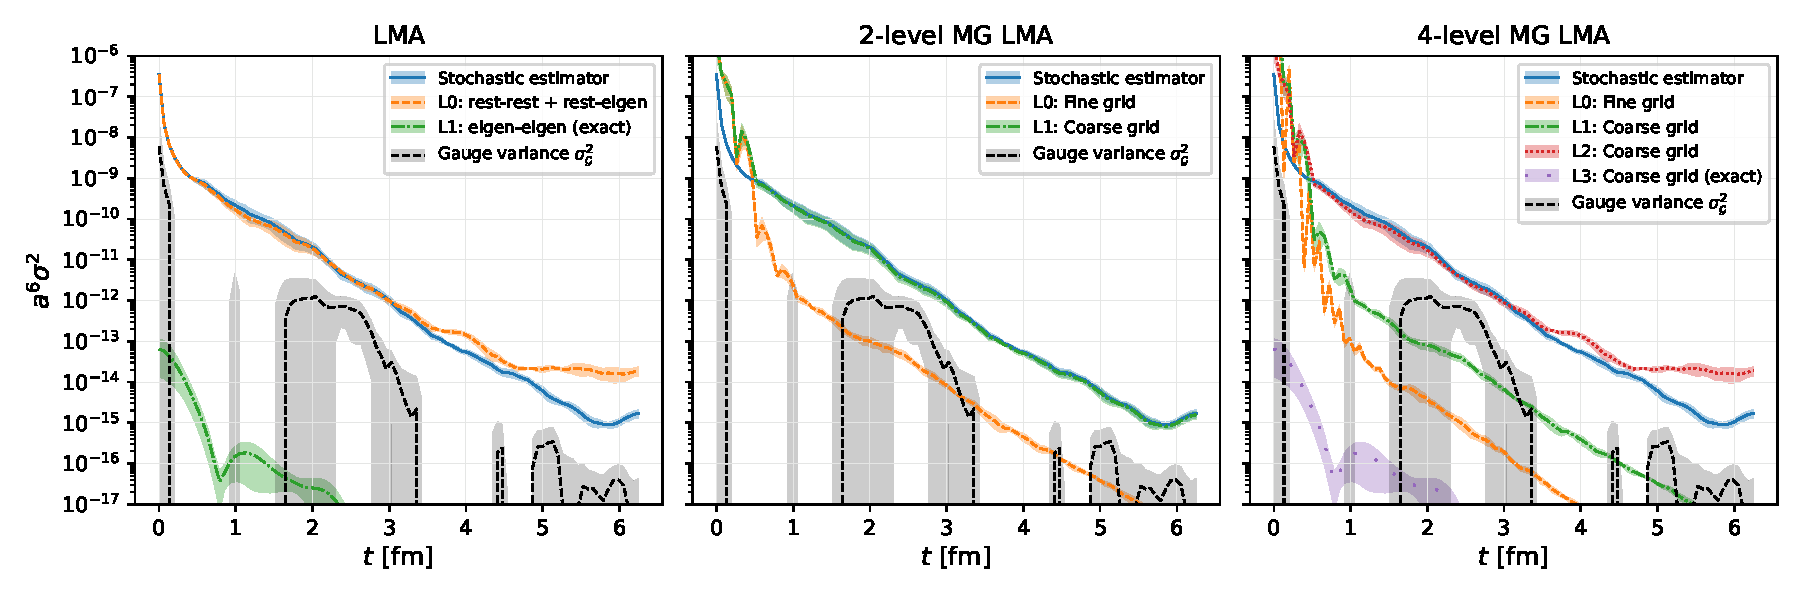
\includegraphics[width=1.0\linewidth]{\dir/img/H7/H7_abs_variance}
\caption{
H7: Absolute total variance \cref{eq:abs:variance} of a single stochastic source.
The left panel shows data for the LMA estimator, center and right show 2-level multigrid and a 4-level multigrid LMA estimator.
The blue solid line represents the pure stochastic estimator without any deflation and the black dashed line indicates the gauge variance of the full correlator. Both appear in all panels for comparison.
}
\label{fig:H7:abs:variance}
\end{figure}

\section{Reaching gauge variance}

In order to determine how many sources are required on every level to reach the gauge variance, we consult the plot series in \cref{fig:E7:var:vs:sources,fig:F7:var:vs:sources,fig:G7:var:vs:sources}.
The required numbers are assembled in \cref{tab:cost}.
The plots show the variance against the number of stochastic sources $\Nst$.
We expect the variance to decrease roughly as $1/\Nst$ (dotted lines in the plots).
The data in the plots are extracted on time-slice $t \approx $ \u{1.3}{\femto \metre}.
This corresponding to the time extent where the signal-to-noise ratio problem starts to be severe~\cite{Kuberski_2023}.

We considered reaching the gauge variance as soon as the line and the gauge variance where consistent with one another.
On most ensembles one single source on the fine-grid is enough -- as explained earlier on F7 the setup was not ideal.
The important point is that the bulk of the variance is captured on the coarse lattices.
Having $\bigO(1000)$ sources on the fine lattice is expensive and infeasible, but on coarse lattices absolutely fine.
For instance the \Ln{2} operator on G7 in the 4-level scheme \cref{fig:G7:var:vs:sources} is a factor \num{512} smaller in its dimension than the \Ln{0} operator.
Inversions on the \Ln{2} lattice are cheaper by about that factor, assuming the same solver algorithm.
It is thus simple to sample that level excessively using \num{1024} sources to push its variance down to the gauge variance.
The cost of these \num{1024} \Ln{2}-inversion is roughly the same as the cost of about \num{2} \Ln{0}-inversions.
On the same lattice, we observe that the LMA estimator basically broke down, because the \Ln{0}-noise it right up with the stochastic estimator, i.e. at the upper bound value with no variance reduction.

\begin{figure}
\centering
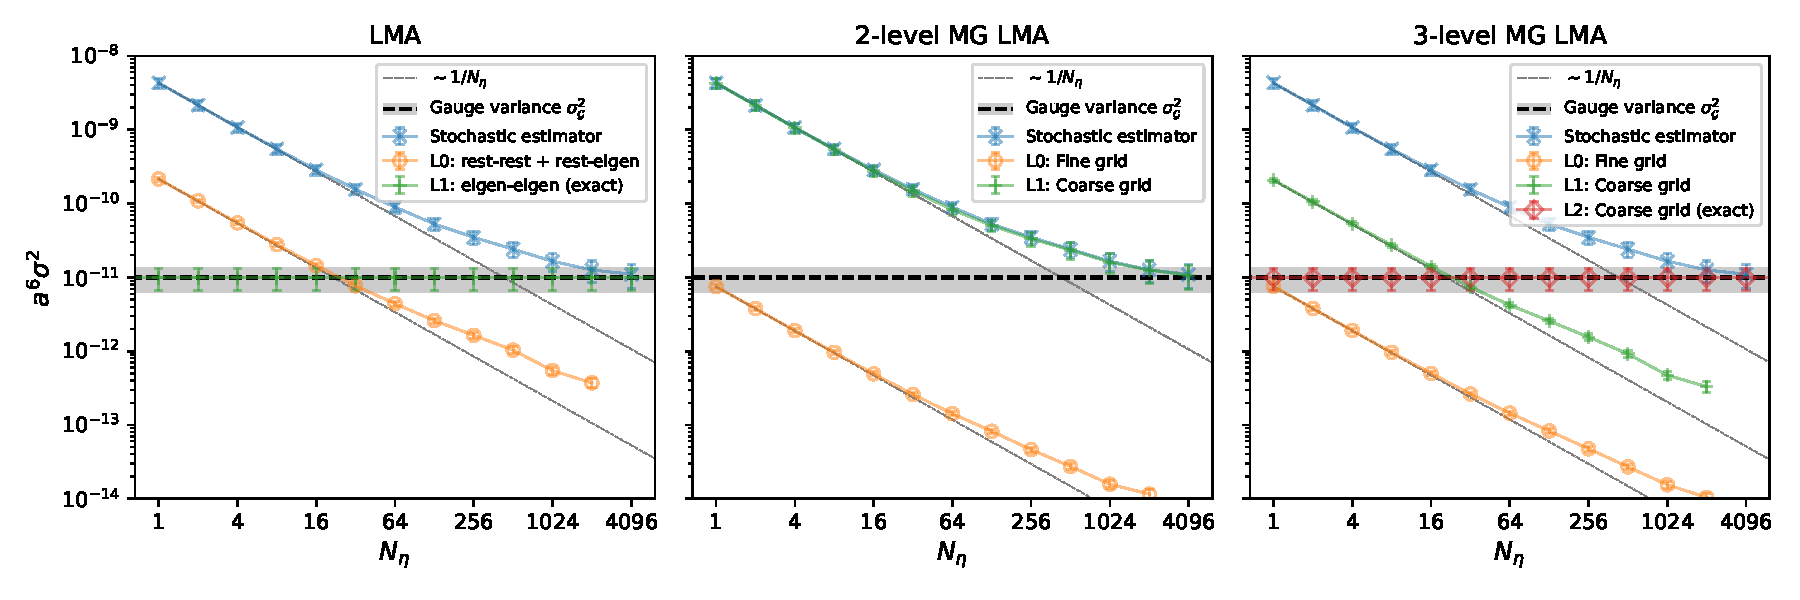
\includegraphics[width=1.0\linewidth]{\dir/img/E7/E7_var_vs_srcs}
\caption{
E7: Absolute total variance \cref{eq:abs:variance} vs. the number of stochastic sources.
The left panel shows data for the LMA estimator, center and right show 2-level multigrid and a 3-level multigrid LMA estimator.
The blue solid line represents the pure stochastic estimator without any deflation and the black dashed line indicates the gauge variance of the full correlator. Both appear in all panels for comparison.
\takenpart
}
\label{fig:E7:var:vs:sources}
\end{figure}

\begin{figure}
\centering
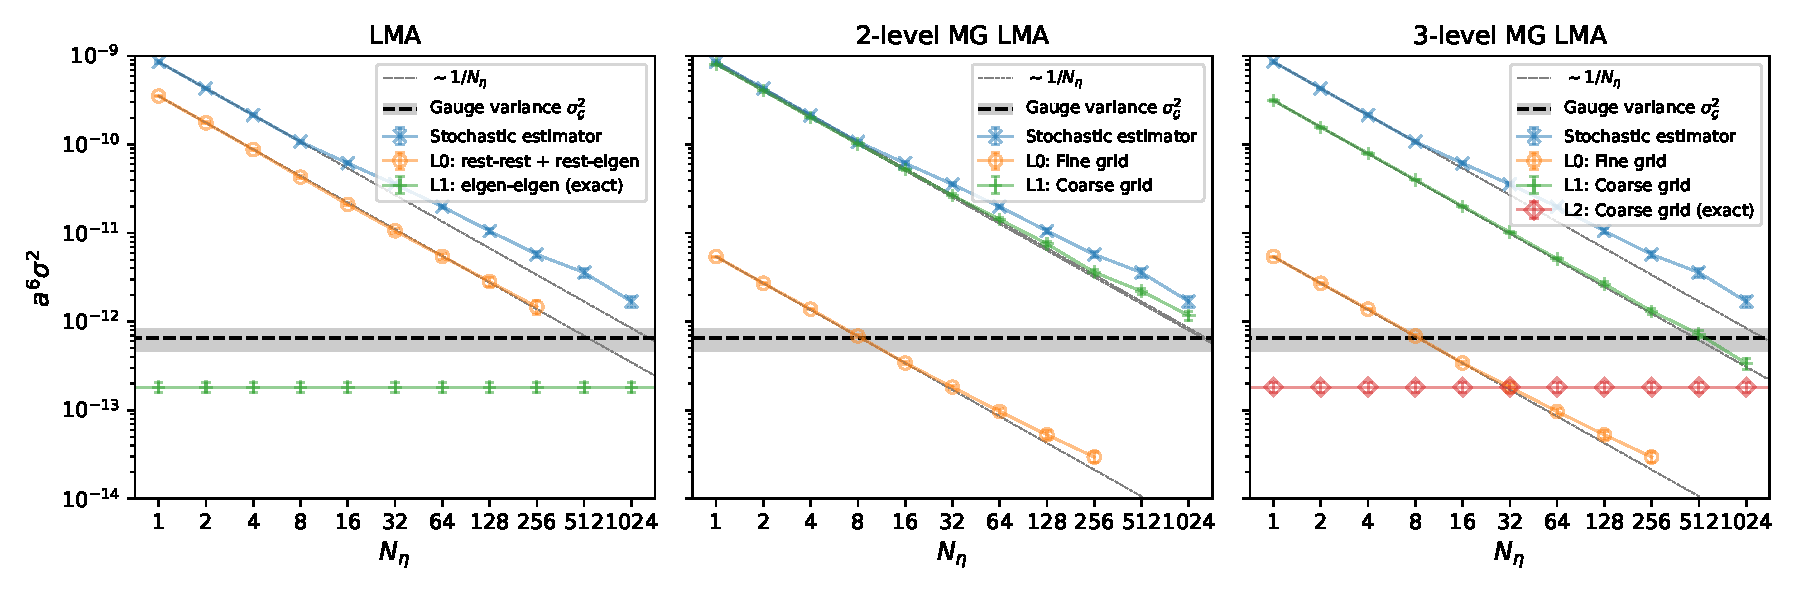
\includegraphics[width=1.0\linewidth]{\dir/img/F7/F7_var_vs_srcs}
\caption{
F7: Absolute total variance \cref{eq:abs:variance} vs. the number of stochastic sources.
The left panel shows data for the LMA estimator, center and right show 2-level multigrid and a 3-level multigrid LMA estimator.
The blue solid line represents the pure stochastic estimator without any deflation and the black dashed line indicates the gauge variance of the full correlator. Both appear in all panels for comparison.
\takenpart
}
\label{fig:F7:var:vs:sources}
\end{figure}

\begin{figure}
\centering
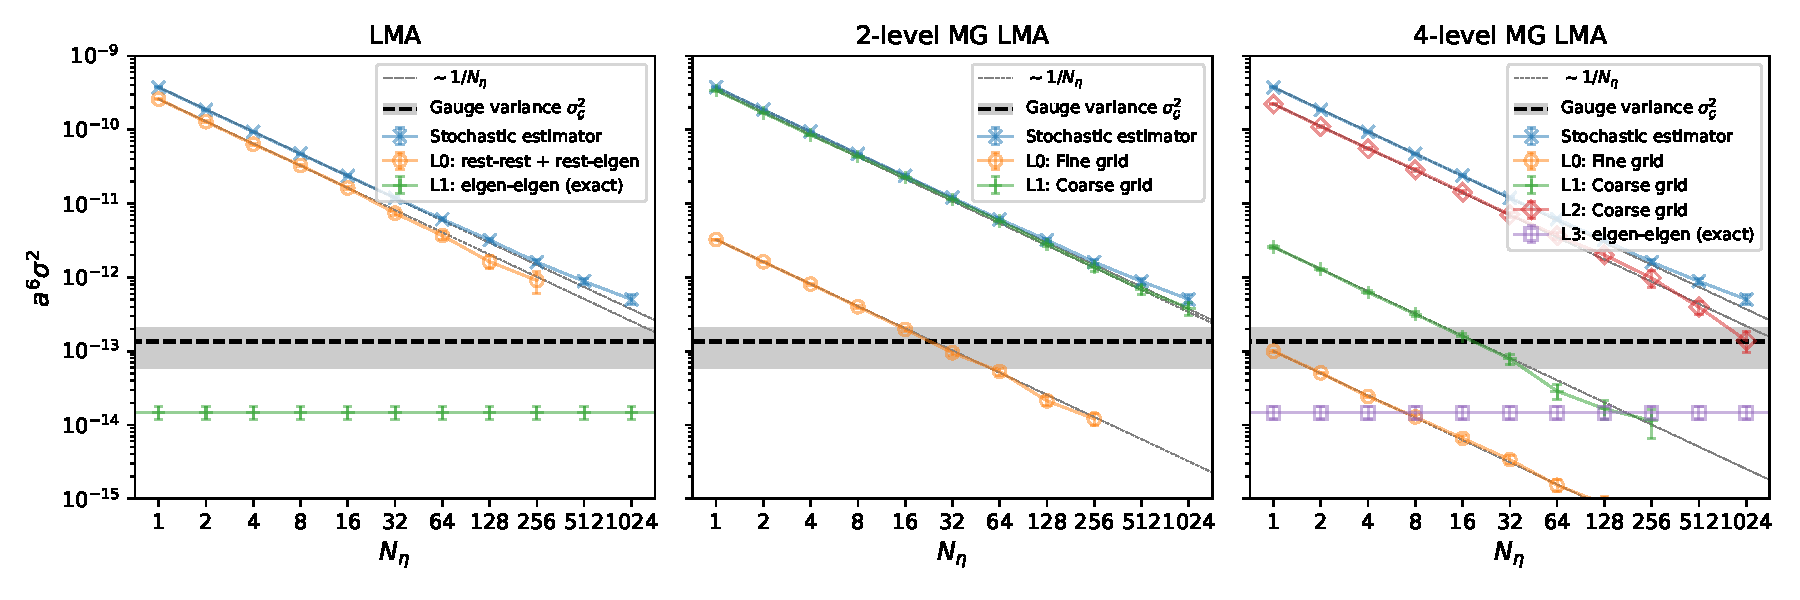
\includegraphics[width=1.0\linewidth]{\dir/img/G7/G7_var_vs_srcs}
\caption{
G7: Absolute total variance \cref{eq:abs:variance} vs. the number of stochastic sources.
The left panel shows data for the LMA estimator, center and right show 2-level multigrid and a 4-level multigrid LMA estimator.
The blue solid line represents the pure stochastic estimator without any deflation and the black dashed line indicates the gauge variance of the full correlator. Both appear in all panels for comparison.
\takenpart
}
\label{fig:G7:var:vs:sources}
\end{figure}

\section{Volume scaling}
\label{sec:numerics:volume:scaling}

Finally, we discuss the volume scaling.
\Cref{fig:var:vs:volume} shows the variance on time-slice $t \approx $ \u{1.3}{\femto \metre} for one single stochastic source on the LMA, 2-level MG LMA and a pure stochastic estimator.
The behavior of the stochastic estimator is straightforward to predict.
Its variance decreases with inversely proportional to the \textit{spatial} lattice volume.
This is expected since we use time-diluted random wall-sources which have support on the spatial volume of their time-slice, that results in an implicit spatial lattice volume averaging of the correlator, see \cref{eq:stoch:C:full:final}.
Thus, the larger lattices result in a reduced variance of the stochastic estimator, because of the spatial lattice volume averaging.

The gauge variance on the other hand is defined in \cref{eq:var:gauge,eq:appendix:gv:formula} as the variance of the full lattice volume averaged correlator \cref{eq:G:corr:volume:averaged} and is thus expected to decrease inversely proportional to the \textit{spacetime} lattice volume.
The usefulness of the pure stochastic estimator is therefore limited, because it chases the gauge variance which decreases faster by a factor of the temporal lattice extent.
Although being a simple method, this is one of the main reasons why it is rarely been used standalone on large lattices close to the physical point.

As already touched upon, we observe that the effect of pure low mode deflation (LMA), as the lattice volume increases, becomes negligible unless one also increases the number of low modes proportional to the volume.
This is apparent in the \Ln{0} line of the left panel.
It even increases in variance and eventually saturates the expected upper bound; the pure stochastic estimator.
The exactly evaluated \Ln{1} term is not of concern, since its variance is bound from above by the gauge variance.

2-level MG LMA on the right panel shows that the \Ln{0} term on the fine grid behaves mostly as $1/L^{3}$.
Deviations of that are due to finite volume effects on the smallest lattice E7.
The time-slice $t \approx $ \u{1.3}{\femto \metre} is already quite close to its maximal extent of \u{2.1}{\femto \metre}.
However, the remaining three data points behave as $1/L^{3}$.
Variances of the \Ln{1} term and the pure stochastic estimator basically coincide.
This is exactly what we aim for with the method.
It shows that independent of the lattice volume, we can capture the bulk of the variance in the cheap-to-evaluate \Ln{1} term on the coarse lattice.
All that remains is to push down the variance of the \Ln{1} term by sampling it with the number of sources as stated in \cref{tab:cost}.

\begin{figure}
\centering
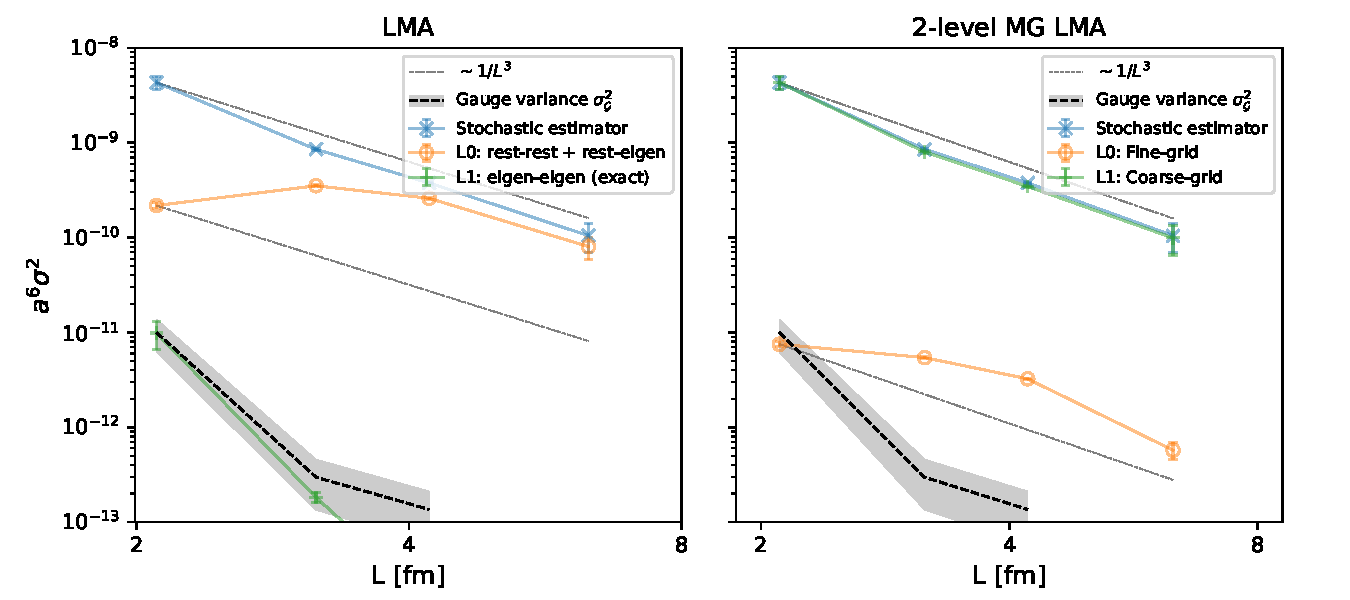
\includegraphics[width=1.0\linewidth]{\dir/img/volume}
\caption{
Absolute total variance \cref{eq:abs:variance} vs. lattice extent $L$.
The left panel shows data for the LMA estimator, whereas the right panel shows a simple 2-level multigrid LMA with equal block size on all lattices, see \cref{tab:lma:estimators}.
The blue solid line represents the pure stochastic estimator without any deflation and the black dashed line indicates the gauge variance of the full correlator. Both appear in both panels for comparison.
\takenfull
}
\label{fig:var:vs:volume}
\end{figure}

\begin{table}[b!]
\begin{threeparttable}
\begin{tabular}{ccccccccc}
\toprule
\multirow{2}{*}{{Ens.}} &
\multirow{2}{*}{{Estimator}} &
\multirow{2}{*}{$\Nc$} &
\multicolumn{4}{c}{$\Nst$} &
\multicolumn{2}{c}{cost} \\
\cmidrule(lr){4-7}
\cmidrule(lr){8-9}
&&& \Ln{0} & \Ln{1} & \Ln{2} & \Ln{3} & meas. & mod. \\
\midrule
E7 & Stochastic   &    & 1024 &         &         &         & $4096$  & $4096$  \\
   & LMA          & 50 & 16   & $\star$ &         &         & $64$    & $64$    \\
   & 2-lvl MG LMA & 50 & 1    & 1024    &         &         & $100.4$ & $12.3$  \\
   & 3-lvl MG LMA & 50 & 1    & 16      & $\star$ &         & $5.5$   & $4.1$   \\
\midrule
F7 & Stochastic   &    & 2048 &         &         &         & $8192$  & $8192$  \\
   & LMA          & 50 & 1024 & $\star$ &         &         & $4096$  & $4096$  \\
   & 2-lvl MG LMA & 50 & 16   & 2048    &         &         & $462.3$ & $80.7$  \\
   & 3-lvl MG LMA & 50 & 16   & 1024    & $\star$ &         & $263.2$ & $72.3$  \\
\midrule
G7 & Stochastic   &    & 4096 &         &         &         & $16384$ & $16384$ \\
   & LMA          & 50 & 2048 & $\star$ &         &         & $8192$  & $8192$  \\
   & 2-lvl MG LMA & 50 & 16   & 2048    &         &         & $557.8$ & $80.7$  \\
   & 4-lvl MG LMA & 50 & 1    & 16      & 1024    & $\star$ & $466.7$ & $14.4$  \\
\bottomrule
\end{tabular}
\begin{tablenotes}\footnotesize
\item[$\star$] The level was evaluated exactly as described in \cref{sec:mglma:coarsest:exact}.
\end{tablenotes}
\caption{\label{tab:cost}
Cost comparison to reach gauge noise of the different estimators used in this document.
The unit of cost is number of fine-grid inversions.
For trivial lattices on the coarsest grid the contribution was calculated exactly and its associated cost is zero.
The actual cost is estimated by direct measurement \cref{tab:cost:imp} and modeled using a performance model discussed in \cref{sec:numerics:performance:model}.
We did not add the cost of generating $\Nc=50$ low modes for multiple reasons. If the number is as small as $50$, one can safely store them to disk and reuse them for different observables.
Their cost is amortized quickly.
As stated multiple times in the text, the LMA estimator requires significantly more modes on the larger lattices to be able to compete with the MG LMA estimator, resulting in a cost increase.
The goal of this document is to compare the two estimators using \emph{equal} resources in terms of low modes and show the volume dependence of both of them when they are held constant.
However, if one insists to add the cost, one can add \numrange{100}{200} to the numbers above.
This amounts to a cost of \numrange{2}{4} inversions per low mode.
% Comparison of the number of stochastic sources used on each level for all schemes and ensembles.
% The associated cost is given in units of the cost of one fine grid inversion.
% This amounts $0.378(2)$, $3.03(1)$ and $12.6(5)$ core-hours for the lattices E7, F7 and G7 respectively, see \cref{tab:cost:imp}.
% For levels where no blocking is used, no stochastic estimator is required and the associated cost is zero.
}
\end{threeparttable}
\end{table}

\section{Cost}

Next, we compare cost of the difference estimators.
A breakdown to reach gauge noise can be seen in \cref{tab:cost}.
We list the three ensembles E7, F7 and G7 with their estimators.
Details about the estimators can be obtained from \cref{tab:lma:estimators}.
\Cref{tab:cost} displays two column for cost; the measured cost and the modeled cost, both in terms of fine-grid inversions.
We decided for this cost metric, because it is machine-independent yet expressive.
A conversion to absolute time to solution (TTS) can be readily made by plugging in the time of a fine-grid inversion on some system of interest.

The measured cost is obtained by direct time-measurements of our own implementation.
At the time of measuring, no multigrid solver was available, therefore the coarsening and the subspaces had to be implemented from scratch.
Clearly an existing performant multigrid implementation is advantageous for a performant implementation of multigrid LMA.

Our own implementation suffered specially on large intermediate lattices.
The reason for this is that we had a very performant solver for the fine-grid inversions; a deflated GCR solver with additional preconditioning in terms of Schwarz-alternating procedure.
On the other hand, the coarse grid solver was a simple even-odd preconditioned GCR.
These two solvers are not on eye-level and thus the performance of our coarse grid inversions was heavily degraded by that fact.

The measured timings are assembled in \cref{tab:cost:imp}, where we note that this table has to be taken with a grain of salt.
For instance on the G7 lattice with a large intermediate \Ln{1} lattice, we see that the \Ln{1} solver needed about \num{30} times more iteration steps than the fine grid \Ln{0} for the same relative residual.
Main reason for that is the difference in preconditioning.
However, it directly results in about three times slower inversions in terms of TTS.
Nevertheless we see clear improvement even with our inefficient coarse grid solver.
In \cref{sec:numerics:coarse:condition} we will show that the coarse Dirac operators are indeed easier to invert in all cases assuming the same solver algorithm is used.

The stochastic estimator in \cref{tab:cost} is our baseline.
It is straightforward to determine its cost in terms of fine-grid inversions; it is read off from \cref{fig:E7:var:vs:sources,fig:F7:var:vs:sources,fig:G7:var:vs:sources} by inspecting where blue line enters the gauge variance error band and multiplying by a factor \num{4}.
We observe an increase in stochastic sources for larger lattices.
As discussed in \cref{sec:numerics:volume:scaling}, we expect the stochastic estimator to degrade in efficiency, because the gauge variance decreases inversely proportional to the lattice volume, whereas for the stochastic estimator it is the spatial lattice volume.

Furthermore, we have evaluated an LMA estimator with $\Nc=50$ low modes on all lattices.
Whereas on the smallest lattice E7 it is very beneficial, decreasing the cost by a factor of \num{64} with respect to the baseline, it becomes less and less significant on the other lattices giving only a speedup of about \num{2}.
Clearly we could make the speedup of this estimator roughly constant by increasing the number of low modes proportional to the lattice volume.
Its cost is determined by counting the number of stochastic sources required on the fine grid to reach gauge variance.

Finally, we inspect the MG LMA estimators.
On the three lattices we used difference multigrid schemes.
The measured and the modeled cost for the coarse grid inversion was calculated using the cost formula
\begin{equation} \label{eq:numerics:cost}
\text{cost} = 4 \sum_{\lvl = 0}^{\Nlvl -1} \frac{\Nst(\Ln{\lvl})}{\ratio(\Ln{\lvl})} \;,
\end{equation}
where $\Nlvl$ is the number of multigrid levels.
The number of stochastic sources used on level $\lvl$, denoted as $\Nst(\Ln{\lvl})$ is read off from the corresponding columns in \cref{tab:cost}.
For the measured cost we read of the ratio $\ratio(\Ln{\lvl})$ from \cref{tab:cost:imp}, which is the dimensionless ratio of the average measured TTS of a fine grid divided by a coarse grid inversion.
The modeled ratio will be discussed separately in \cref{sec:numerics:performance:model}.
The factor \num{4} comes from the fact that we use spin-diagonal random wall-sources on all levels, which amounts one inversion per spin degree of freedom.

The smallest lattice E7 shows two estimators; a two-level scheme using the $\Nc=50$ low modes to create a subspace with block size $8^4$ (see \cref{tab:lma:estimators}) and a three-level scheme that is the combination of the LMA estimator with the two-level scheme.
This lattice is of special interest, because we see that the two-level MG LMA estimator is worse than the traditional LMA estimator using our implementation.
Even though the remaining \num{16} fine-grid sources decreased to a single one, we had to introduce \num{1024} sources on the coarse grid as opposed to none.
Using our inefficient coarse inverter, this trade-off resulted in a net cost increase.
However when instantiating a third level these \num{1024} coarse grid sources decreased to only \num{16}.
We emphasize that this is the same factor \num{64} as the LMA estimator had over the stochastic one, which is not a coincidence, when inspecting \cref{fig:E7:var:vs:sources}.
Deflation of pure low modes had the effect of pushing down the \Ln{0} variance of the LMA estimator (see \cref{fig:E7:var:vs:sources} right).
In the exact same way we pushed down the \Ln{1} variance (see \cref{fig:E7:var:vs:sources} center) by deflating it with the pure low modes (see \cref{fig:E7:var:vs:sources} left).
However, the intermediate non-trivial lattice between the fine grid and the trivial lattice has the effect of both pushing down the \Ln{0} noise to the gauge variance and decreasing the required source on \Ln{1} to \num{16}.

We go on discussing the intermediate lattice F7, where the MG LMA scheme was not chosen ideally.
The LMA estimator is not beneficial anymore, making the three-level scheme only marginally better than the two-level one.
With ideally chosen coarse grids, we would expect its cost in terms of fine-grid inversions to be in between the cost of E7 and G7.
This could have been reached with another intermediate coarse lattice of block size of either $6^4$ or $4^4$ with respect to \Ln{0}, similar as to the four-level scheme of G7.

Finally the largest lattice fully analyzed is G7.
We have employed the same two-level scheme as for the other lattices, but additionally ran a four-level scheme with another non-trivial coarse lattice and traditional LMA as final level.
The final level on this lattice did not contribute and could have been removed safely without cost impact.
However the final lattices -- if trivial -- were not considered in the cost estimation, because these are just 100 dimensional all to all contractions, see \cref{eq:mglma:coarsest:exact}.

The cost of the MG LMA compared to the LMA estimators decreased by introducing non-trivial coarse lattices, over which we sample.
Even with our modest implementation we observe huge speedups over the plain stochastic, but also over the LMA estimator with a constant number of low modes.

\begin{table}[b!]
\begin{tabular}{ccccrrr}
\toprule
{Ens.} & 
{Type} & 
{Lattice} & 
{Blk.} &
{TTS [core-h]} &
%{$\ratio = \textrm{coarse/fine}$} &
Ratio $\ratio$&
{\# iteration} \\
\midrule
E7              & fine   & $64  \times 32^3$ &       & 0.378(2)  & $1.0$       & $35.7(2)$    \\
                & coarse & $8   \times 4^3$  & $8^4$ & 0.009     & $42.6(2)$   & $140.5(3)$   \\
\midrule                                                                        
F7              & fine   & $96  \times 48^3$ &       & 3.03(1)   & $1.0$       & $43.77(15)$  \\
                & coarse & $12  \times 6^3$  & $8^4$ & 0.15      & $20.6(1)$   & $337.6(1.3)$ \\
\midrule                                                                        
G7              & fine   & $128 \times 64^3$ &       & 12.6(5)   & $1.0$       & $46.53(23)$  \\
                & coarse & $32  \times 16^3$ & $4^4$ & 42(2)     & $0.29(2)$   & $1417(22)$   \\
                & coarse & $16  \times 8^3$  & $8^4$ & 0.76(5)   & $16.6(1.2)$ & $502(6)$     \\
\bottomrule
\end{tabular}
\caption{\label{tab:cost:imp}
Average cost in terms of core-hours for an inversion on the fine and coarse grids.
The block size is indicated in the fourth column, empty corresponds to the fine lattice.
The time to solution (TTS) is reported in core-hours and $\ratio$ is the ratio of the TTS of a fine grid solve divided by a coarse grid solve.
$\ratio$ is used as input for the measured cost calculation using \cref{eq:numerics:cost} in \cref{tab:cost}.
The last column reports the average number of iterations required for the solver to converge.
It emphasizes the unequal solvers used on the different grids.
We note that one should take care when comparing timings from one lattice to another, because they were taken on different machines with different node setups.
% Cost of inversion of the fine and coarse grid operators in core-hours.
% For the fine grid a very efficient implementation is available in contrast to our probably suboptimal coarse grid solver.
% The relative cost to the fine grid inversion \worktodo{todo} is used to the compute the cost in \cref{tab:cost}.
% 
}
\end{table}

\subsection{Condition of coarse Dirac operators}
\label{sec:numerics:coarse:condition}

We will continue motivating the performance model by investigating the condition number of coarse Dirac operators.
The success of the method crucially depends on the fact that the coarse Dirac operators $\onlvl{D}{\lvl}$ are better conditioned than the fine grid one.
This is because the convergence behavior of Krylov subspace solvers depends on the eigenvalue distribution and the condition number of the operator to solve.
For instance, for conjugate gradient (CG) the number of iteration steps scales as~\cite{shewchuk1994introduction}
\begin{equation}
\Niter \sim \bigO\left(\sqrt{\kappa(D)}\right) \log\left(\frac{1}{\epsilon}\right) \;,
%\Niter \leq \frac{1}{2} \sqrt{\kappa(D)} \log\left(\frac{2}{\epsilon}\right) \;,
\end{equation}
where $\epsilon$ is the precision of the solution $\psi$ after $\Niter$ iterations and $\kappa(D)$ is the condition number of the operator $D$,
\begin{equation}
\epsilon = \frac{\norm{D \psi - \eta}}{\norm{\eta}} \;,
\qquad
\kappa(D) = \frac{\lambda_{\text{max}}}{\lambda_{\text{min}}} \;,
\end{equation}
with $\lambda_{\text{max}}$ and $\lambda_{\text{min}}$ the smallest and largest magnitude eigenvalues of $D$.
Even though for other Krylov subspace solvers there is no closed formula for the iteration count as for CG, the rule of smaller condition number implies smaller iteration count is generally applicable.

To empirically show this, we used the G7 ensemble, where we studied a 4-level scheme, thus \num{4} Dirac operators, all with different dimensions.
Their approximate condition number as well as their iteration counts to solve a random right-hand side to a certain precision was plotted in \cref{fig:coarse:condition} as a function of the dimension over the complex numbers.
The leftmost operator is the diagonal Dirac operator emerging in an LMA scenario, see \cref{eq:sd:lma:diagonal:dirac}, and the rightmost one is the operator on the fine-grid with dimension $12 V$.
The two intermediate data points correspond to the \Ln{1} and \Ln{2} operators for the 4-level MG LMA estimator of G7 in \cref{tab:lma:estimators}.

Our assumptions from above are clearly met by \cref{fig:coarse:condition}; the smaller the operator dimension the smaller the condition number and by this the smaller the iteration count.
It is thus save to assume -- with the same solver algorithm on all levels -- that coarser levels are cheaper to perform solves on than finer ones.

% \begin{figure}
% \centering
% 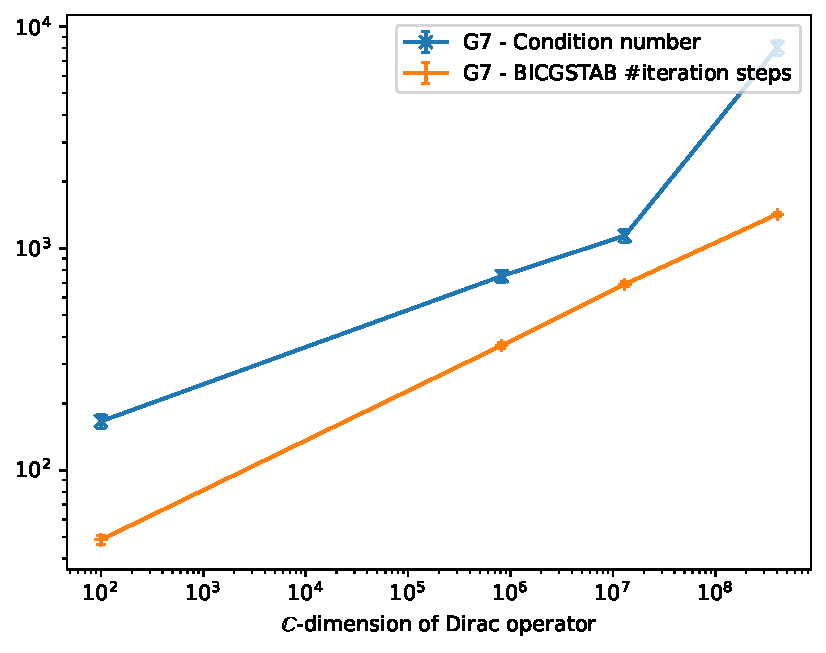
\includegraphics[width=0.6\linewidth]{\dir/img/coarse_condition}
% \caption{\worktodo{caption}.}
% \label{fig:coarse:condition}
% \end{figure}

\begin{figure}
\centering

\subfloat[Coarse operator condition]{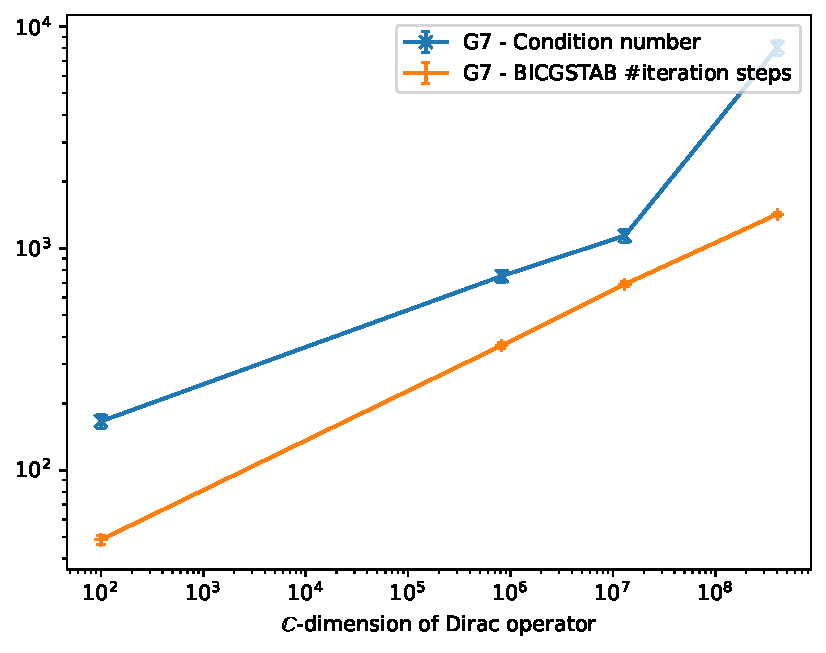
\includegraphics[width=0.49\textwidth]{\dir/img/coarse_condition}\label{fig:coarse:condition}}
\hfill
\subfloat[Memory bandwidth model]{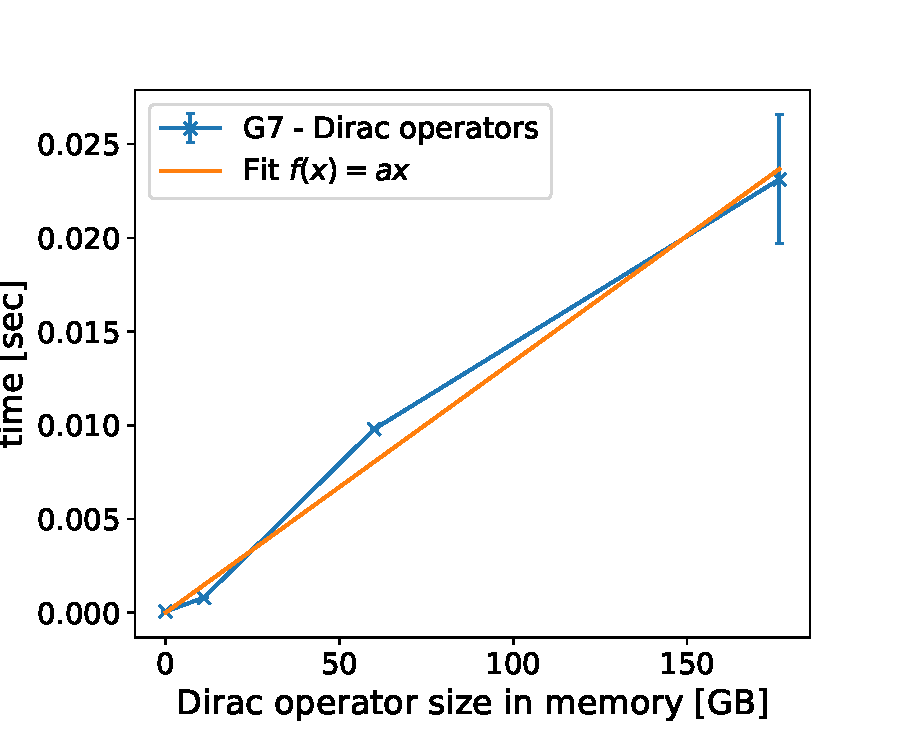
\includegraphics[width=0.49\textwidth]{\dir/img/coarse_tts_vs_memory}\label{fig:coarse:memory}}

\caption{\worktodo{regenerate plots}
(a) Estimated condition number and average number of iteration steps for a Biconjugate gradient stabilized solve (BiCGSTAB) vs. the dimension of the operator on G7. \takenfull
(b) Time for one application of a fine- or coarse-grid Dirac operator vs. their memory footprints on G7.
}
\label{fig:coarse}
\end{figure}

\subsection{Performance model}
\label{sec:numerics:performance:model}

Based on the insights of the previous section, we will quantify the improvement factor of a coarse grid solve compared to a fine grid one.
This will give us an estimate for the ratio $\ratio$ to use in the cost formula \cref{eq:numerics:cost} to obtain a cost estimate as if we have used the same solver algorithm on all levels, i.e. as if we had access to all components of a performant multigrid solver.

The high coarse grid iteration count of our disadvantageous implementation is refuted considering numerical results in \cref{sec:numerics:coarse:condition}.
A second problem emerges as one increases the dimension of the coarse operators, because they -- even though having the same sparsity pattern as the fine one -- are less sparse in general, since they usually have more color degrees of freedom.

Sparse matrix vector multiplication is the dominant kernel in a Krylov solver.
It is a memory bandwidth bound operation.
The time of a Dirac operator application is proportional to its size in memory, see \cref{fig:coarse:memory}.
The rightmost data point in the plot is not the fine grid operator as one might assume, but the \Ln{1} operator.
In case of coarse operators from the 4-level scheme of G7, the \Ln{1} operator is about \num{3} times larger in memory than the fine grid Dirac operator from which it is constructed.
Besides the different solver algorithms on fine and coarse grids, this fact is responsible for the degradation of performance of our implementation.
On first sight this poses a clear problem.
In the following we will argue that this problem is in fact neither an issue and nor a performance limiter.

We will start with formalizing the cost of a single inversion involving operator $K$.
Motivated by \cref{fig:coarse:memory}, our choice for the unit of cost is memory traffic,
\begin{equation} \label{eq:numerics:perf:cost:single:rhs}
\cost(K) = \iter(K) \left[ \mem(K) + (N_{K} + 1) \cdot \mem(\psi) \right]
\end{equation}
where $\iter(K)$ denotes the average number of iterations required to solve a linear system of equation with the operator $K$ for some right-hand side and some fixed relative residual.
The memory traffic produced by applying an operator $K$ or reading a field $\psi$ is denoted by $\mem(K)$ and $\mem(\psi)$ respectively.
The number $N_K$ depends on the sparsity pattern of the operator, its implementation and the machine\footnote{If $K$ is a nearest neighbor stencil, the right-hand side may be read multiple times, depending on the sparsity patter of the stencil, implementation thereof and cache hierarchy and size of the machine. If $K=D$ the Wilson-Dirac operator in 4D spacetime, $N_K = N_D = 1-9$, because for every lattice point, we need to read all direct neighbors in \num{8} directions including the point itself, compare \cref{eq:Dw:QCD+QED}. In the worst case this amounts \num{9} reads of the same point, but if cache reusage patterns are favorable this number will be smaller.}.
We assume that every solver iteration consists of one application of $K$, which involves one read of $K$, $N_K$ reads and one write of the right-hand side $\psi$.
We have neglected further operations on the vectors, like scalar products, norms or axpys\footnote{This stands for $a \vect{x} + \vect{y}$, scalar times vector plus vector, "a x plus y". It resembles the BLAS level-1 routine call family of the same name.}, because we assume the operator memory traffic to dominate.

With the performance model defined in \cref{eq:numerics:perf:cost:single:rhs}, we are clearly confronted with the issue mentioned before.
% This would result in a estimator for the speedup of
% \begin{equation}
% \speedup(1) = \frac{ }{}
% \end{equation}
Therefore we continue with the definition of the cost of $\Nrhs$ simultaneous solves as
\begin{equation}
\cost(K, \Nrhs) = \iter(K) \left[ \mem(K) + (N_{K} + 1) \Nrhs \cdot \mem(\psi) \right] \,.
\end{equation}
This equation is motivated by the fact that when applying the operator $K$ to $\Nrhs$ right-hand sides simultaneously, the operator has to be read only once instead of $\Nrhs$ times, if implemented in a multiple right-hand sides fashion~\cite{Boyle:2024pio}.
Meaning the operator can operate on many right-hand sides at the same time.
This turns matrix-vector multiplications into matrix-matrix multiplications improving temporal cache locality and increasing arithmetic intensity.
%It can be implemented in a way where the operator $K$ is read from memory only once although applied to $\Nrhs$ vectors.

Finally we can define the speedup of a coarse grid solve of $\coarse{K}$ with respect to a fine grid solve of $K$ as the ratio of their cost
\begin{equation}
\speedup(\Nrhs)
= \frac{
   \iter(K) \left[ \mem(K) + (N_{K} + 1) \Nrhs \cdot \mem(\psi) \right]
}{
   \iter(\coarse{K}) \left[ \mem(\coarse{K}) + (N_{\coarse{K}} + 1) \Nrhs \cdot \mem(\coarse{\psi}) \right]
} \;.
\end{equation}

With one right-hand side assuming $\mem(K) \gg \mem(\psi)$ we find
\begin{equation} \label{eq:numerics:speedup:bad}
\speedup(1)
\approx \frac{ \iter(K) }{ \iter(\coarse{K}) }
  \frac{ \mem(K) }{ \mem(\coarse{K}) } \;.
\end{equation}
This is exactly what we observe with our modest implementation: on some coarse grids both the iteration count and the memory traffic blow up making the inversion slow compared to the fine grid.

On the other hand using a multiple right-hand side (mRHS) solver in the asymptotic limit of many right-hand sides, we find instead
\begin{equation}
\lim_{\Nrhs \to \infty} \speedup(\Nrhs)
= \frac{ \iter(K) }{ \iter(\coarse{K}) }
\frac{ (N_{K} + 1) }{ (N_{\coarse{K}} + 1) }
  \frac{ \mem(\psi) }{ \mem(\coarse{\psi}) } \;.
\end{equation}
We emphasize that the dependence of the memory traffic of the operator $\mem(K)$ dropped, compare \cref{eq:numerics:speedup:bad}.
Conservatively we will assume the iteration count to not change from fine to coarse grid, i.e. $\iter(K) = \iter(\coarse{K})$, even though \cref{sec:numerics:coarse:condition} suggested $\iter(K) > \iter(\coarse{K})$, but quantifying that factor is not trivial.

The coarse operator $\coarse{K}$ has the same sparsity pattern than the fine one.
This suggests $N_{K} \approx N_{\coarse{K}}$ although spin and color degrees of freedom differ making $\coarse{K}$ usually less sparse than $K$.
This might result in a less efficient implementation of the coarse operator.
For simplicity, we will assume equally-efficient implementations, $N_{K} = N_{\coarse{K}}$.

The memory traffic produced by the coarse and fine-grid fields are easily worked out.
They are proportional to the dimension,
\begin{align}
\mem(\psi) &= 12 V \cdot \sizeof(Float) \;, \\
\mem(\coarse{\psi}) &= \coarse{N}_s \coarse{\Nc} \coarse{V} \cdot \sizeof(Float) \;.
\end{align}
The irrelevant size of the datatype in bytes, \sizeof(Float), cancels in the ratio and since the produced memory traffic of an inversion $\cost(K)$ is proportional to the TTS of the same, we can interpret the speedup as ratio
\begin{equation} \label{eq:numerics:speedup:good}
\ratio(\Ln{\lvl})
= \lim_{\Nrhs \to \infty} \speedup(\Nrhs)
\approx \frac{ \mem(\psi) }{ \mem(\coarse{\psi}) }
= \frac{12 V}{ \coarse{N}_s \coarse{\Nc} \coarse{V} } \;.
\end{equation}
Thus the cost ratio in our performance model is just the ratio of dimensions.

For the determination of the modeled cost in \cref{tab:cost} we used \cref{eq:numerics:cost} with \cref{eq:numerics:speedup:good} as ratio $\ratio$.
The values are assembled in \cref{tab:cost:model}.
A mRHS solver is expected to be computationally even more beneficial on the coarse grids than on the fine grid when considering cache effects, because coarse spinors may fit in cache easier.

\begin{table}
\begin{tabular}{ccccccr}
\toprule
{Ens.} &
{Type} &
{Level} &
{Lattice} &
{$N_s$} &
{$N_c$} &
Ratio $\ratio$ \\
\midrule
E7              & fine   & \Ln{0} & $64  \times 32^3$ & 4 & 3  & $1.0$    \\
                & coarse & \Ln{1} & $8   \times 4^3$  & 2 & 50 & $491.52$ \\
\midrule                                                                        
F7              & fine   & \Ln{0} & $96  \times 48^3$ & 4 & 3  & $1.0$    \\
                & coarse & \Ln{1} & $12  \times 6^3$  & 2 & 50 & $491.52$ \\
\midrule                                                                        
G7              & fine   & \Ln{0} & $128 \times 64^3$ & 4 & 3  & $1.0$    \\
                & coarse & \Ln{1} & $32  \times 16^3$ & 2 & 50 & $30.72$  \\
                & coarse & \Ln{2} & $16  \times 8^3$  & 2 & 50 & $491.52$ \\
\bottomrule
\end{tabular}
\caption{\label{tab:cost:model}
Ratio $\ratio$ for the modeled cost of the different MG LMA estimators used in this document.
}
\end{table}



% \begin{figure}
% \centering
% 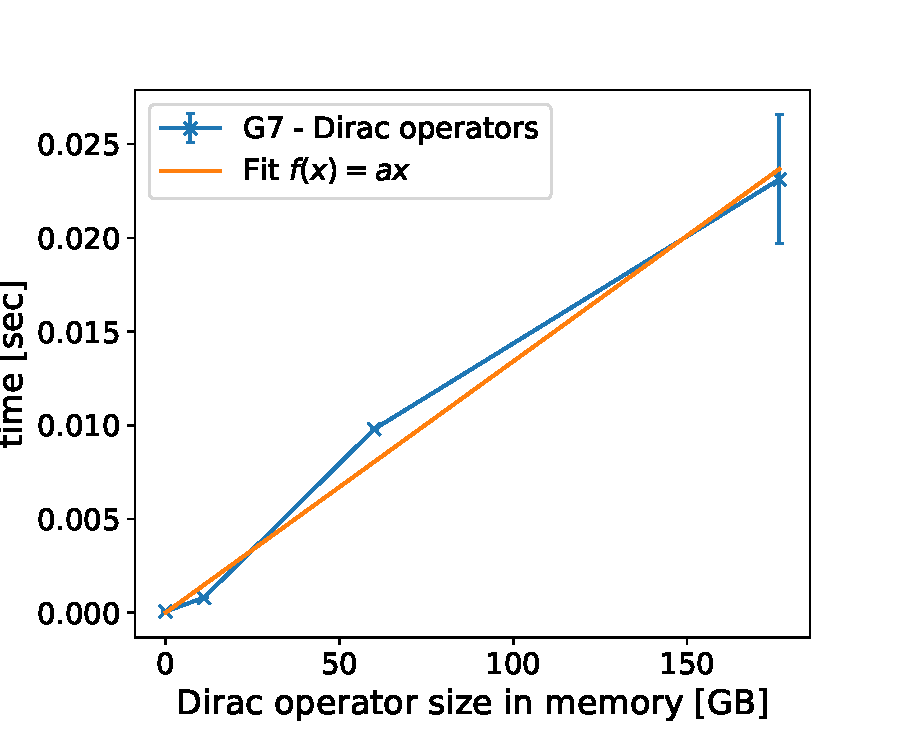
\includegraphics[width=0.6\linewidth]{\dir/img/coarse_tts_vs_memory}
% \caption{
% Time for one application of a fine- or coarse-grid Dirac operator (y-axis) vs. their memory footprints on G7.
% }
% \label{fig:coarse:memory}
% \end{figure}


%The modeled cost was also obtained using \cref{eq:numerics:cost}, but with a different ratio $\ratio$.

\section{Summary}
\label{sec:numerics:summary}

We have shown the consistency and performance of the new method, we refer to as multigrid low-mode averaging as compared to the plain stochastic and the traditional low-mode averaging estimators.
The most important finding in this chapter is that the achieved variance reduction is flat in the lattice volume as opposed to traditional sampling schemes.
Due to the good overlap with the true low-mode subspace, we observe speedups of more than an order of magnitude compared to the plain stochastic and LMA estimators.

The majority of the variance is contained in the cheap parts, whereas the expensive remainder shows suppressed variance contribution.
This hierarchical sampling scheme leads to a flat scaling behavior of required number of low modes, leading to a linear volume-scaling in computational cost.
Since coarse operators are better conditioned than fine ones, sampling coarse subspaces is always less expensive than sampling the fine ones, keeping the cost factor under control.

% \worktodo{
%    * We showed, the method works for O(a)-improved Wilson-Clover fermions
%    * Subspace captures the low mode behavior, i.e. the majority of noise
%    * All variance in cheap coarse piece
%    * Variance suppression on expensive remainder
%    * Hierarchy of stochastic sampling on all levels
%    * LMA and MG LMA
%    * Reaching gauge variance
%    * Volume scales linearly, most important message! LMA does not!
%    * Cost is under control
%    * Coarse operators are better conditioned
%    * perf model assuming MRHS solvers
% }
